\documentclass[UTF8]{ctexart}
\usepackage{amsmath}
\usepackage{amssymb}
\usepackage{amsthm}
\usepackage{graphicx}
\usepackage{CJK}
\usepackage{float}
\usepackage{mdframed}
\providecommand{\abs}[1]{\lvert#1\rvert}
\providecommand{\norm}[1]{\lVert#1\rVert}
\providecommand{\ud}[1]{\underline{#1}}

\newmdtheoremenv{thm}{Theorem}
\newmdtheoremenv{lemma}[thm]{Lemma}
\newmdtheoremenv{fact}[thm]{Fact}
\newmdtheoremenv{cor}[thm]{Corollary}
\newtheorem{eg}{Example}
\newtheorem{ex}{Exercise}
\newmdtheoremenv{defi}{Definition}
\newenvironment{sol}
  {\par\vspace{3mm}\noindent{\it Solution}.}
  {\qed \\ \medskip}

\newcommand{\ov}{\overline}
\newcommand{\ca}{{\cal A}}
\newcommand{\cb}{{\cal B}}
\newcommand{\cc}{{\cal C}}
\newcommand{\cd}{{\cal D}}
\newcommand{\ce}{{\cal E}}
\newcommand{\cf}{{\cal F}}
\newcommand{\ch}{{\cal H}}
\newcommand{\cl}{{\cal L}}
\newcommand{\cm}{{\cal M}}
\newcommand{\cp}{{\cal P}}
\newcommand{\cs}{{\cal S}}
\newcommand{\cz}{{\cal Z}}
\newcommand{\eps}{\varepsilon}
\newcommand{\ra}{\rightarrow}
\newcommand{\la}{\leftarrow}
\newcommand{\Ra}{\Rightarrow}
\newcommand{\dist}{\mbox{\rm dist}}
\newcommand{\bn}{{\mathbb N}}
\newcommand{\bz}{{\mathbb Z}}

\newcommand{\expe}{{\mathsf E}}
\newcommand{\pr}{{\mathsf{Pr}}}


\setlength{\parindent}{0pt}
%\setlength{\parskip}{2ex}
\newenvironment{proofof}[1]{\bigskip\noindent{\itshape #1. }}{\hfill$\Box$\medskip}

\theoremstyle{definition}
\newtheorem{problem}{Problem}
\newtheorem*{problem*}{Problem}

\pagenumbering{gobble}

\begin{document}

\title{CS477 Combinatorics: Homework 7}
\author{于峥 518030910437}
\date{\today}

\maketitle

在下面的这些游戏中,$n$个人中每个人随机独立地被戴上红蓝两色帽子之一,概率各$1/2$。每个人可以看到所有别人的颜色,但是看不到自己的颜色。他们需要同时猜各自帽子的颜色。

\begin{problem}
A {\em strategy} can be formalized as a sequence of functions
\[
(f_1, f_2, \dots, f_n),
\]
where each $f_i$ is a function $\{0, 1\}^{n-1} \to \{0, 1\}$.

How many strategies are there in total?
\begin{sol}
    $f_i$有$2^{2^{n-1}}$种选择,因此共有$2^{n2^{n-1}}$策略。
\end{sol}
\end{problem}

\begin{problem}
Consider the following strategy: For each person, if she sees that the colours of the other hats are all the same, she guesses 0 for herself, otherwise she guesses 1.

For $n=3$, draw the strategy on the hypercube, by labeling the vertices and giving directions to each edge. 
\begin{sol}
    \begin{figure}[ht]
        \centering
        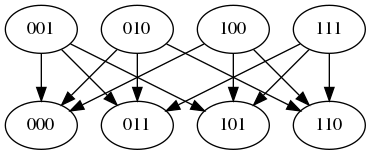
\includegraphics[scale=0.36]{figures/hc.png}
        \caption{Hypercube}
        \label{fig:label}
    \end{figure}
\end{sol}
\end{problem}

\begin{problem}
In this problem, their goal is: either every player guesses correctly, or every player gives a wrong guess.

How many different strategies do they have to achieve the goal? Prove your answer. 
\begin{sol}
    由于我们希望所有人都正确或错误,所以如果两个人看到相同的01串,必然作出相同的选择。这意味着代表
    策略的超立方体上每个点要么只有入度,要么只有出度。注意到一个只有入度的点的邻点必然
    只有出度。所以我们可以把超立方体黑白染色,让黑点只有入度。白点只有出度。 假设立方体上一个
    点已经确定了颜色,那么和这个点最短距离为奇数的点异色,偶数为同色。而超立方体可以二染色。
    所以染色方法只有两种。
\end{sol}
\end{problem}

\begin{problem}
In this problem, their goal is: make sure $m$ players guesses her colour correctly.

What is the maximum $m$ in terms of $n$? Prove your answer. 
\begin{sol}
    如果我们希望任何情况下都至少有$m$人正确,那么意味着策略超立方体中每个点的入度至少为
    $m$。而整个图的出入度和为$n2^n$, 因此$m \leq \frac n 2$。并且$m=\left\lfloor\frac n 2 \right\rfloor$
    是可以取到的。我们先将图黑白染色,然后对于图中的两点$u, v$。如果$u,v$不同的
    那一位为奇数且$x$为黑色或者不同的那一位为偶数且$x$为白色那么有$u \rightarrow v$,否则
    反向。这样构造是一定满足要求的。
    
    我们考虑如果立方体$G$中我们只留下那些二进制位之间只有一位不同,并且这一位在偶数上。
    那么这个图$H$和$G/H$每个点的度数至少为$\left\lfloor\frac n 2 \right\rfloor$。
    我们让$H$中黑点连的边全为入边,$G/H$黑色连的边全为出边,白色点相反。那么把这两个图合并起来
    后每个点的入度将为$\left\lfloor\frac n 2 \right\rfloor$。

\end{sol}
\end{problem}

\end{document}


